% Para qué usamos en el MDCM el fuzzy? Para manejar Uncertainty y subjectivity.

% Information integration (aggregation)

% Distance measures

% Preference relations

% \signal{
%     Entropy desde el punto de vista de la posibilidad es el que más específico es. Es máxima si el conjunto tiene un unico punto, entonces sabes que es super especifico, ese concepto corresponde a ese unico punto y a nada más. Desde el punto de vista de la informacion es cuanto más informativo, mayor entropía. Desde el punto de vista de la probabilidad es cuanto más te distingue los sucesos: la delta de dirac tiene mínimo y la uniforme máximo o algo así era. 
%     Eso lo tengo que repasar.
%     }\\


% Cosas para mencionar sobre fuzzy en MCDM:

% \signal{OWA operators, y sus generalizaciones. Orness, andness, orlike y andlike.

% Entropía de un OWA, quantifiers

% Fuzzy implication operators para la importancia de los OWA

% Fuzzy ratings, que es como tener 2 fuzzy weights y así incorporas la linguistic variable.

% Fuzzy reasoning: tienes fuzzy rules y las agregas con un OWA por ejemplo. Puedes hacer la implicación y luego agregar o agregar y luego hacer la implicación.

% MICA operators es la clase más general de operators en fuzzy modeling.

% 3 mecanismos de MISO fuzzy system

% Compositional rule of inference

% Generalized method of case inference rule

% Interdependencia de los criterios!

% % Lo de que la importancia es relativa, puedo tener unos criterios sí y otros no y tal y que eso me cambie el grado de importancia.}

% \signal{Aquí pensaba definir agregación en general como una función. Luego presento los OWAs y sus variaciones. Hasta aquí sí que lo tengo claro.

% Pero para seguir, quería simplemente poner los métodos que vaya a usar en la aplicación práctica del tema 3. No sé si un fuzzy TOPSIS o ELECTRE o alguno de esos que tengo en el diagrama de arriba. O si por el contrario puedo continuar con generalizaciones de los OWA pero eso ya sería meterme otra vez con fuzzy measures y acabaría en la integral de Choquet, de Sugeno o de Shilkret o alguna de esas. También otro método sería meterme en lo de reglas de inferencia, ya que he empezado con lo de Pavelka y el razonamiento aproximado, podría ser interesante igual.}

% \section{Fuzzy Aggregation}
\label{sec:fuzzy_aggregation}

% In the context of multi-criteria decision making, after evaluating each alternative against every criterion, the next logical step is to combine these individual assessments into a single, comprehensive value for each alternative. This process is known as aggregation and would belong to the \emph{Value Measurement Methods} strategy presented in section \ref{sec:crisp_methods}. 

% % \signal{Include here the definition of aggregation function in a \begin{definition}}

% An aggregation function takes a collection of numerical inputs, representing the performance scores of an alternative, and maps them to a single output value. This overall score should ideally be a meaningful representation of the inputs, allowing for a final ranking of the alternatives. \signal{Weighted Arithmetic Mean (WAM)
% Median, Minimum, and Maximum
% Geometric and Harmonic means
% Ordered Weighted Averaging (OWA) functions
% Fuzzy integrals\footnote{like the Choquet and Sugeno integrals and say very briefly how these relate to the concept fuzzy measure concept discussed in \ref{sec:fuzzy_measures}.}}\\






In the context of multi-criteria decision making, after evaluating each alternative against every criterion, the next logical step is to combine these individual assessments into a single, comprehensive value for each alternative. This process is known as aggregation\footnote{In some books, especially in control systems' literature, it might be found under the name of \textit{defuzzification}, since it involves converting the fuzzy information into a single value for making a decision.} and would belong to the \emph{Value Measurement Methods} strategy presented in section \ref{sec:crisp_methods}. The formalism and concepts discussed in this section are primarily based on the books \cite{beliakov2023discrete} and \cite{xu2015uncertain}.

\begin{definition}[Aggregation Function] \label{def:aggregation_function}
An aggregation function is a function $f: [0, 1]^n \to [0, 1]$ that satisfies the following two properties for any input vectors $\mathbf{x}, \mathbf{y} \in [0, 1]^n$:
\begin{romanenum}
    \item \textbf{Boundary Conditions:} The function preserves the boundaries of the interval:
    \[f(0, 0, \dots, 0) = 0\text{ and }f(1, 1, \dots, 1) = 1\]
    \item \textbf{Monotonicity:} The function is jointly non-decreasing in all its arguments:
    \[\text{If }\mathbf{x} \le \mathbf{y}\text{ (meaning }x_i \le y_i \forall i=1, \dots, n\text{), then }f(\mathbf{x}) \le f(\mathbf{y})\]
\end{romanenum}
\end{definition}

An aggregation function takes a collection of numerical inputs, representing the performance scores of an alternative, and maps them to a single output value. This overall score should ideally be a meaningful representation of the inputs, allowing for a final ranking of the alternatives. It should be noted that the choice of non-decreasing monotonicity rather than non-increasing is purely conventional. This convention aligns with the intuitive principle that higher membership values indicate more desirable properties of alternatives. Although the inverse ordering could be considered for ranking alternatives downwards, the \textit{higher is better} paradigm is generally more natural and thus preferred. Common examples of aggregation functions include: weighted (arithmetic, geometric or harmonic) means, median, minimum, maximum, ordered weighted average (OWA) or fuzzy integrals\footnote{Integrals defined using non-additive fuzzy measures, such as the Choquet and Sugeno integrals.}.\\

A simpler approach like the weighted average has a fundamental limitation due to its weights being fixed to specific criteria. This does not allow for modeling the decision maker's attitude, such as optimism or pessimism, towards the performance scores themselves (see example \ref{ex:why_owa} below). To address this, the Ordered Weighted Averaging (OWA) operator, introduced by Yager in \cite{YagerOWA}, provides a more flexible framework. The core innovation of the OWA operator is that it disassociates the weights from the criteria and instead associates them with the ordered positions of the values. That is, weights are assigned based on a value's rank (e.g., to the highest value, the second highest, and so on) rather than to the criterion it came from.\\

\begin{example}\label{ex:why_owa}
    Consider a homebuyer evaluating two houses. House A represents a ``high-risk, high-reward" option, while House B represents a balanced safe option. A standard Weighted Average (WA) barely distinguishes between them, regardless of the chosen weights, as it does not consider whether an attribute has a higher or lower value. The OWA operator enables modeling an optimistic buyer who focuses mainly on the best features, or a pessimistic buyer who prioritizes avoiding weak points.

    \[W_A = (0.2, 0.5, 0.3), \quad W_{\text{opt}} = (0.7, 0.2, 0.1), \quad W_{\text{pess}} = (0.1, 0.2, 0.7) \]
    \begin{align*} 
    \text{House A: } (0.9, 0.8, 0.1)\quad  \Rightarrow \quad \text{WA} = 0.61,\quad  \text{OWA}_{\text{opt}} = 0.80, \quad  \text{OWA}_{\text{pess}} = 0.32 \\
    \text{House B: } (0.6, 0.6, 0.6) \quad \Rightarrow \quad \text{WA} = 0.60,\quad   \text{OWA}_{\text{opt}} = 0.60,  \quad \text{OWA}_{\text{pess}} = 0.60
    \end{align*}
    The results demonstrate how OWA captures decision attitude: the optimist favors House A due to its high scores, while the pessimist prefers House B due to House A's single low score. The weighted average fails to capture this nuance, producing nearly identical scores.
\end{example}

\begin{definition}[Ordered Weighted Averaging (OWA) Operator]
Let $(a_1, a_2, \dots, a_n)$ be a collection of values to be aggregated. The OWA operator is a mapping $\text{OWA}: \mathbb{R}^n \to \mathbb{R}$ defined by a weighting vector $W = (w_1, w_2, \dots, w_n)$ such that $w_i \in [0, 1]$ and $\sum_{i=1}^{n} w_i = 1$. The aggregated value is given by:
\[
\text{OWA}(a_1, a_2, \dots, a_n) = \sum_{j=1}^{n} w_j b_j
\]
where $b_j$ is the $j$-th largest value in the collection $(a_1, a_2, \dots, a_n)$.
\end{definition}

The key to the OWA operator's flexibility lies in the determination of the weighting vector $W$. By changing the distribution of the weights, one can model a wide spectrum of aggregation behaviors. For instance, an optimistic decision maker, who focuses on the best outcomes, would assign higher weights to the first components of the vector $W$, thereby giving more importance to the highest-ranked values ($b_1, b_2, \dots$). Conversely, a pessimistic decision maker would assign higher weights to the last components, emphasizing the worst-performing criteria. A standard arithmetic mean is recovered by setting all weights equal, $w_j = 1/n$. This ability to model the decision maker's attitude is a significant advantage over the simple weighted average. A fundamental quantity in this regard is the \textit{orness}\footnote{Its dual, \textit{andness}, can also be defined as $1-\text{\textit{orness}}$, but it does not provide any additional information.}, which quantifies the degree of optimism of the operator. It is calculated as \[\text{orness}(W) = \sum_{j=1}^{n} w_j \frac{n-j}{n-1}\] 
An orness of 1 corresponds to pure optimism (like the maximum operator, where $w_1=1$), an orness of 0 corresponds to pure pessimism (like the minimum operator, where $w_n=1$), and an orness of 0.5 reflects a neutral attitude (like the arithmetic mean).

\begin{remark}
    It should be noted that OWA operators and their direct variants rely on an additive measure of importance, as the weights must sum to one and the aggregated importance of any subset of criteria equals the sum of its individual weights. This framework assumes that the criteria are preferentially independent. It does not capture more complex interactions between criteria, such as synergy or redundancy (where the combined effect of two criteria is greater or lower than their sum). Modeling such relationships requires non-additive fuzzy measures and more complex aggregation tools, like the Choquet or Sugeno integrals, which are not studied in this work.\\
\end{remark}


The OWA operator has inspired numerous extensions and variations, such as the Ordered Weighted Geometric (OWG) operator for contexts where a multiplicative aggregation is more suitable, and hybrid operators like the Induced OWA (IOWA) and the Combined Weighted Averaging (CWA), which seek to reintroduce the importance of the criteria themselves alongside the attitudinal weighting. 



\subsection{Assigning weights}

% The process of defining the weights can be guided by several methods. More intuitively, weights can be derived from linguistic quantifiers, such as "most", "at least half", or "about three". These quantifiers can be mathematically modeled to generate a corresponding weighting vector $W$, allowing the decision maker to specify their aggregation strategy in a natural and understandable way.\\


The process of defining the weights for the OWA operator is a critical step that directly models the decision-maker's attitude towards risk and trade-offs. Several methods have been developed to guide this process and can be categorized by the type of information they elicit from the decision maker.



\paragraph{Linguistic Quantifiers}
Perhaps the most intuitive method for defining OWA weights is through the use of linguistic quantifiers. It relies on a quantifier function, which models the degree of satisfaction associated with a given proportion of criteria meeting a standard and is often expressed in natural language with words like ``most" or ``at least half", into a weighting vector. 

\begin{definition}[Linguistic Quantifier]
    A function $Q: [0, 1] \to [0, 1]$ is a linguistic quantifier suitable for generating OWA weights if it is monotonically non-decreasing and satisfies the boundary conditions $Q(0) = 0$ and $Q(1) = 1$.
    \end{definition}

From this function, we can derive a set of OWA weights $w_j$ for an aggregation of $n$ items by mapping the $j\text{-th}$ criterion to the $j/n$ proportion and using the following formula:
    \begin{equation}
        w_j = Q\left(\frac{j}{n}\right) - Q\left(\frac{j-1}{n}\right) \quad \text{for } j=1, \dots, n
        \label{eq:quantifier_weights}
    \end{equation}
Since $Q(0)=0$ and $Q(1)=1$, the sum of the increments (weights) is always $1$ (it is a telescoping sum) and monotonicity assures weights are non-negative, producing a valid OWA weighting vector. As illustrated in Figure \ref{fig:quantifier_weights}, a steeper part of the curve $Q(r)$ yields larger weights, while a flatter part yields smaller weights.\\





\begin{figure}[!ht]
    \centering
    % Generated from the python script previously provided.
    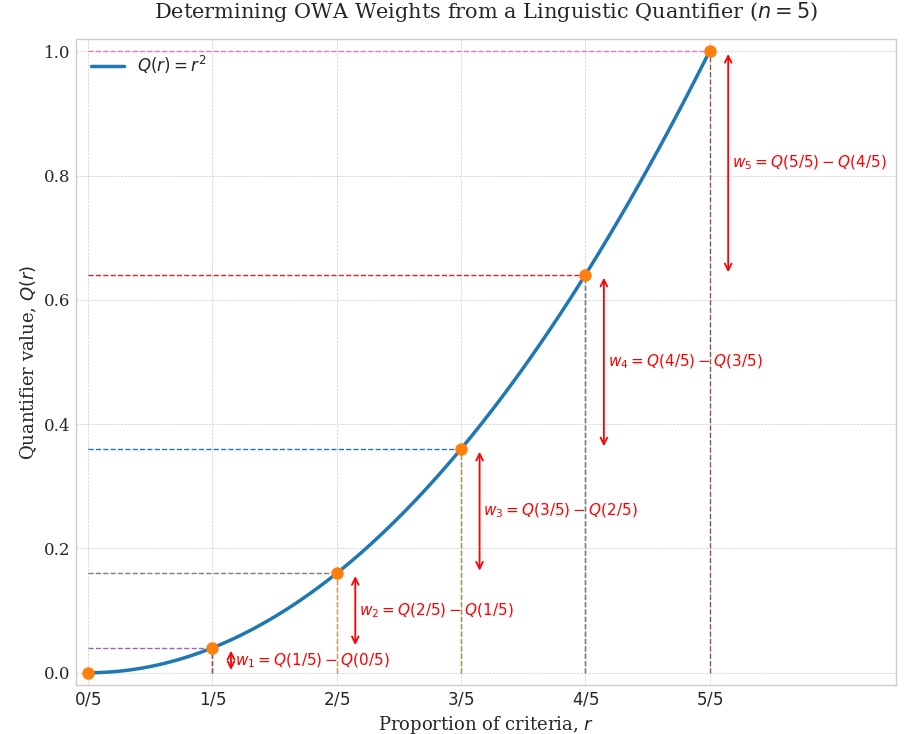
\includegraphics[width=0.65\textwidth]{ch2/figures/linguistic_quantifier_weights.png}
    \caption{Graphical determination of OWA weights from a quantifier function, illustrated with $Q(r) = r^2$ for $n=5$. Each weight $w_j$ is the vertical increase of the function $Q$ over the interval $[\frac{j-1}{n}, \frac{j}{n}]$. A steeper curve assigns more weight to higher-ranked criteria.}
    \label{fig:quantifier_weights}
\end{figure}

An intuitive way to understand a quantifier function for a fixed number of desired weights $n$ is to interpret it as a piecewise function, where each piece has the same length of $1/n$.\footnote{In general, any number $n$ could be used with any quantifier function, so it is not ``fixed". But as $n$ increases, $j/n$ proportions change, and with them, the ranges of the pieces.} Then, the increment in the y-axis along the j-th piece (in $[\frac{j-1}{n}, \frac{j}{n}]$), corresponds to the j-th weight $w_j$. \\


\begin{example}[Modeling with Quantifiers]
    Different linguistic concepts can be modeled by choosing an appropriate function for $Q(r)$. All these examples are plotted in Figure \ref{fig:quantifier_examples}.
    \begin{itemize}
        \item \textbf{``All'':} The simplest quantifier is $Q(r) = r$. Using Equation \ref{eq:quantifier_weights}, this yields weights $w_j = \frac{j}{n} - \frac{j-1}{n} = \frac{1}{n}$ for all $j$. This corresponds to the simple arithmetic mean, where all criteria are weighted equally.
        \item \textbf{``At least half'':} This can be modeled by a crisp step function: $Q(r) = 0$ for $r < 0.5$ and $Q(r) = 1$ for $r \ge 0.5$. For $n=5$, this would generate the weighting vector $W=(0, 0, 1, 0, 0)$, placing all importance on the median value.
        \item \textbf{``Some":} Focuses on having just some good performing criteria (optimistic decision-maker). This is modeled with a concave quantifier like $Q(r) = \sqrt{r}$. A steeper curve for small $r$ assigns more weight to the highest-ranked inputs. For $n=5$, this generates the vector $W \approx (0.45, 0.18, 0.14, 0.12, 0.11)$. Here, the highest weight $w_1$ is given to the best score, reflecting an optimistic, risk-seeking attitude.

        \item \textbf{``The majority'':} Focuses on not having too low-performing criteria, the majority is good enough (pessimistic or risk-averse decision-maker). This is modeled with a convex quantifier like $Q(r) = r^2$. For $n=5$, this generates the vector $W=(0.04, 0.12, 0.20, 0.28, 0.36)$. The weights increase for lower-ranked criteria, placing more importance on the lower-valued inputs and reflecting a pessimistic attitude.
        
        \item \textbf{The Window-Type Quantifier:} This models instructions like "ignore the best and worst scores and average the middle ones." For $n=5$, using a window quantifier that averages the middle 50\% of scores:
        \[ Q(r) = \begin{cases} 0 & \text{if } r \le 0.25 \\ 2r - 0.5 & \text{if } 0.25 < r \le 0.75 \\ 1 & \text{if } r > 0.75 \end{cases} \]
        This generates weights where the middle-ranked scores have non-zero weights while the extreme scores are ignored.
    \end{itemize}
    \end{example}


\begin{figure}[!ht]
    \centering
    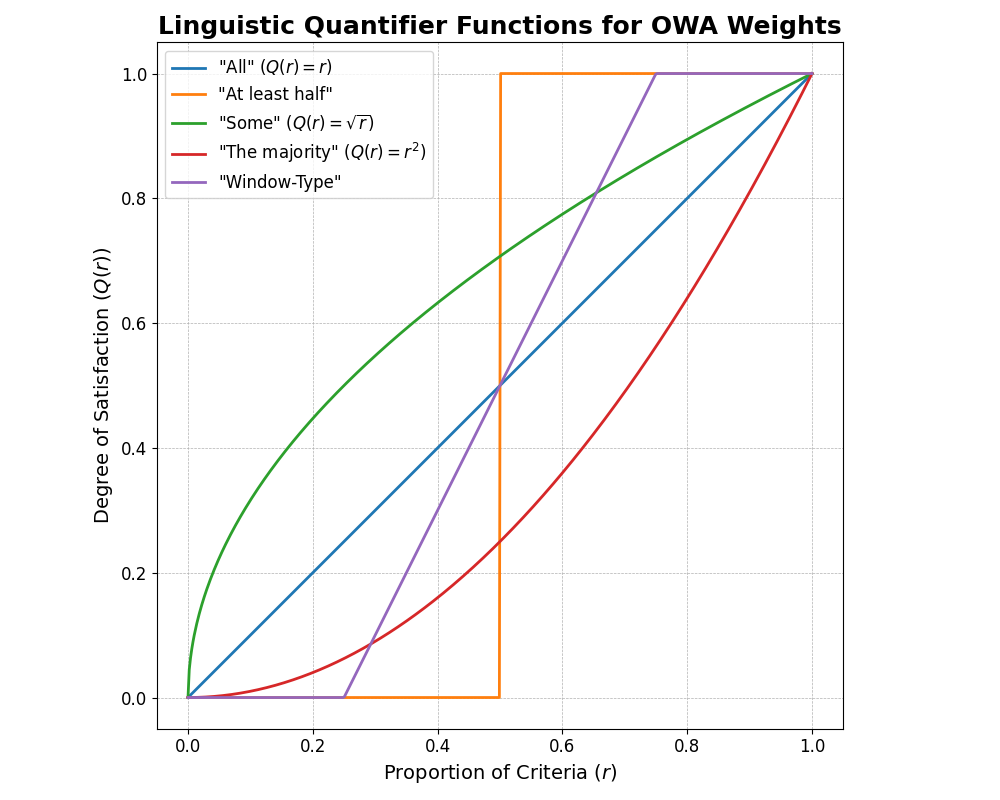
\includegraphics[width=0.8\textwidth]{ch2/figures/Quantifiers_examples.png}
    \caption{Examples of different linguistic quantifiers.}
    \label{fig:quantifier_examples}
\end{figure}
    

The definition above describes what is formally known as a regular non-decreasing quantifier. Fuller presents in \cite[ch.~2]{FULLER2} a complete taxonomy of quantifiers that includes as well: non-increasing quantifiers, which are completely equivalent to the non-decreasing ones and do not provide any advantages, and unimodal ones. The latter is non-monotonic and models concepts like "about two" or "around half." These concepts cannot be represented by a standard OWA operator using the quantifier method because they require negative weights to penalize having a number of non-zero criteria different from the required. 


\paragraph{Defining an Orness Level}

In many cases, a decision-maker may not be able to articulate a specific quantifier but can express a general degree of optimism. The \textbf{orness} measure, as defined in section \ref{sec:fuzzy_aggregation}, directly captures this attitude. This method involves the decision-maker specifying a desired orness level, $\alpha \in [0, 1]$, and then finding a weight vector $W$ that satisfies this preference.\\

However, the equation $\text{orness}(W) = \alpha$ is under-determined. Multiple weight vectors can yield the same orness level. For example, for an orness of $\alpha = 0.5$ and $n=10$, both the mean operator ($w_j = 0.1$ for all $j$) and a polarized operator ($w_1 = 0.5, w_{10} = 0.5$, and other weights zero) satisfy the condition. To resolve this ambiguity, a second principle is needed to select a single, representative weight vector.

\begin{enumerate}[label=(\roman*)]
    \item \textbf{Yager's Power-Quantifier Method}
    
    A direct and systematic way to generate weights from a given orness $\alpha$ is to use a specific family of quantifier functions. Yager proposed using the basic unit monotone increasing quantifier $Q(r) = r^a$, where the exponent $a$ is derived from the desired orness. The orness of this quantifier is given by $\text{orness}(Q) = \int_0^1 r^a dr = \frac{1}{a+1}$. By setting this equal to $\alpha$, we can solve for $a$:
    \begin{equation}
        a = \frac{1}{\alpha} - 1, \quad \text{for } \alpha \in (0, 1)
    \end{equation}
    This method provides a direct, non-optimization-based way to generate a smooth, regular set of weights that systematically reflect the chosen level of optimism. Notice that in the limits $\alpha \in \{0,1\}$, it becomes the minimum or the maximum, so there is no need to compute the weights in those cases.

    \item \textbf{Maximizing Entropy}
    
    Another approach is to formulate an optimization problem. To resolve the ambiguity, we seek the weight vector that, for a given orness, is maximally non-specific or least biased. This is achieved by maximizing the Shannon entropy of the weights. Intuitively, this method finds the most dispersed (similar to the uniform distribution, which has the highest entropy) weight distribution that still satisfies the decision-maker's attitudinal preference. The problem is formulated as:
    \begin{equation}
    \begin{aligned}
        & \text{maximize}   & & H(W) = -\sum_{j=1}^{n} w_j \ln(w_j) \\
        & \text{subject to} & & \text{orness}(W) = \alpha \\
        &                   & & \sum_{j=1}^{n} w_j = 1, \quad w_j \ge 0
    \end{aligned}
    \end{equation}
    This constrained optimization problem has a unique optimal weighting vector $W$ for a given $n$ and $\alpha$. The proof for existance and uniqueness of an optimal solution to this problem can be found in \cite[Sec.~2.3]{FULLER2}.
\end{enumerate}

\paragraph{Maximizing Inter-criteria Variance}
The underlying principle is that a criterion's importance is related to the information it provides for distinguishing between alternatives. This approach assigns higher weights to criteria that show greater variance in performance scores across alternatives. The intuition is that a criterion where all alternatives perform similarly (low discriminative power) is not useful for ranking and should receive a low weight. Conversely, a criterion with high score variation is highly discriminating and thus more important. After normalizing the decision matrix, the weight for criterion $j$ is calculated as:
\begin{equation}
    w_j = \frac{\sum_{i=1}^{n} \sum_{k=1}^{n} |r_{ij} - r_{kj}|}{\sum_{l=1}^{m} \sum_{i=1}^{n} \sum_{k=1}^{n} |r_{il} - r_{kl}|}
\end{equation}
where $r_{ij}$ is the normalized performance score of alternative $i$ on criterion $j$. This method is entirely data-driven and provides an objective basis for weight determination when subjective preferences are unavailable or undesirable.